\documentclass{beamer}
\usetheme{Madrid}

\usepackage{amsmath, amssymb, amsthm}
\usepackage{graphicx}
\usepackage{listings}
\usepackage{gensymb}
\usepackage[utf8]{inputenc}
\usepackage{hyperref}
\usepackage{gvv}

\begin{document}

\title{Mentor PROJECT}
\author{EE23BTECH11016 - Aditi Dure$^{*}$}
\date{}
\frame{\titlepage}

\begin{frame}
\frametitle{Multiplexing in Cellular Communication}
\begin{figure}
	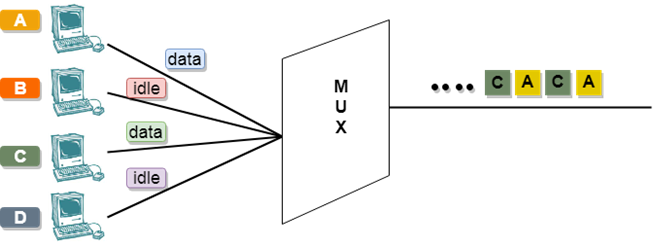
\includegraphics[scale = 0.5]{figs/multiplexing.png}
	\caption{Multiplexing}
\end{figure}
-- a technique used in telecommuniation and data transmission \\
-- efficient use of resources \\
-- optimising bandwidth
\end{frame}

\begin{frame}{allowframebreaks}
\frametitle{Types of Multiplexing}
There are mainly five types of division multiplexing methods as follows:
                \begin{enumerate}
                        \item Time Division Multiplexing
                        \item Frequency Division Multiplexing
                        \item Space Division Multiplexing
                        \item Code Division multiplexing
                        \item Wavelength Division Multiplexing
                \end{enumerate}
The following slides will cover first three Multiplexing Tehniques.
\end{frame}

\begin{frame}
\frametitle{Time Division Multiplexing}
	\begin{figure}
		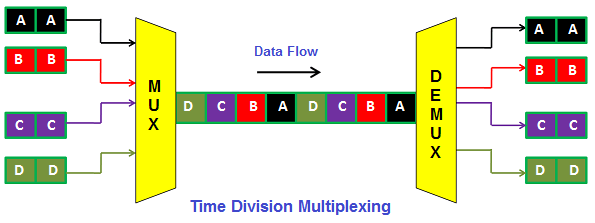
\includegraphics[scale = 0.5]{figs/tdm.png}
		\caption{TDM}
	\end{figure}
\end{frame}
\begin{frame}
\frametitle{TDM -- Key Points}
-- Time Slot Allocation \\
-- Sequencial Transmission  \\
-- Fixed or Variable Length Slots \\
-- Efficient Utilisation of Time \\
-- Examples \\
\end{frame}
\begin{frame}
\frametitle{Frequency Division Multiplexing}
	\begin{figure}
		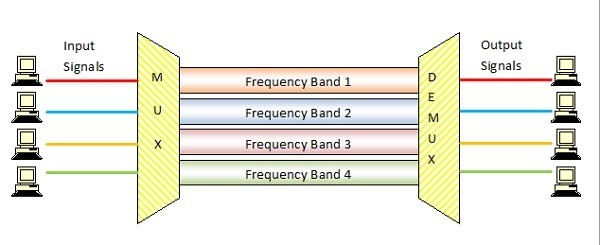
\includegraphics[scale = 0.5]{figs/fdm.jpg}
		\caption{FDM}
	\end{figure}
\end{frame}
\begin{frame}
\frametitle{FDM -- Key Points}
-- Frequency Allocation \\
-- Independent Channels \\
-- Efficient use of Spectrum \\
-- Commonly used Alalog Communication \\
-- Examples \\
\end{frame}
\begin{frame}
\frametitle{Space Division Multiplexing}
\begin{figure}
	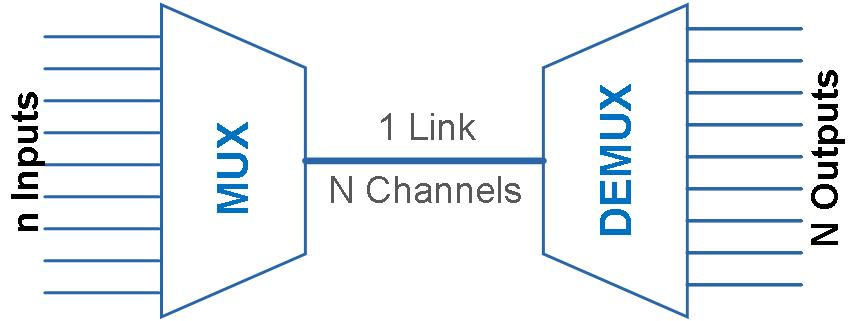
\includegraphics[scale = 0.5]{figs/sdm.jpg}
	\caption{SDM}
\end{figure}
\end{frame}

\begin{frame}
\frametitle{SDM -- Key Points}
-- Multiple Spacial Paths \\
-- Spacial Seperation \\
-- Independent Transmission \\
-- Application in Optial Fiber Communication \\
-- MIMO technology \\
-- Efficiency and Capacity \\
-- Examples \\
\end{frame}
\end{document}
